% compile with pdflatex (twice): Linux Libertine for text and Bera Mono for code
% storyline: story.md; full pages of the earlier decks via \cpa{page} (figures/CPA.pdf) and \nextgen{page}
% (figures/NextGeneration.pdf)
\documentclass[aspectratio=1610,14pt]{beamer}
\usepackage[T1]{fontenc}
\usepackage[utf8]{inputenc}
\usepackage{libertine}
\usepackage[libertine]{newtxmath}
\usepackage[scaled=0.88]{beramono}
\usepackage{listings}
\usepackage{tikz}
\usetikzlibrary{calc,fit,shapes.callouts,shapes.geometric,arrows.meta,positioning}

% the look of the earlier decks: plain white, bold serif titles at the top left,
% blue concepts, red problems, green answers, purple citations
\usefonttheme{serif}
\usefonttheme{professionalfonts}
\setbeamertemplate{navigation symbols}{}
\setbeamertemplate{footline}{\hfill{\color{black!60}\normalsize\insertpagenumber\,/\,\insertdocumentendpage}\hspace*{0.25cm}\vspace*{0.2cm}}
\setbeamertemplate{itemize items}{\textbullet}
\setbeamertemplate{itemize subitem}{--}
\setbeamertemplate{enumerate items}{\insertenumlabel)}
\setbeamersize{text margin left=0.8cm,text margin right=0.8cm}
\setbeamerfont{frametitle}{series=\bfseries,size=\fontsize{17}{20}\selectfont}
\setbeamercolor{frametitle}{fg=black}
\setbeamercolor{structure}{fg=black}
\setbeamercolor{normal text}{fg=black}
\setbeamertemplate{frametitle}{\vspace*{0.3cm}\insertframetitle\par}
\definecolor{cblue}{RGB}{0,0,255}
\definecolor{cred}{RGB}{255,0,0}
\definecolor{cgreen}{RGB}{0,166,60}
\definecolor{cpurple}{RGB}{128,0,128}
\newcommand{\bad}[1]{\textcolor{cred}{#1}}
\newcommand{\good}[1]{\textcolor{cgreen}{#1}}
\newcommand{\concept}[1]{\textcolor{cblue}{#1}}
\newcommand{\cit}[1]{\textcolor{cpurple}{#1}}

% a page of an earlier deck as a full slide
\newcommand{\fullpage}[2]{{\usebackgroundtemplate{\includegraphics[page=#2,width=\paperwidth,height=\paperheight]{figures/#1.pdf}}
  \begin{frame}\end{frame}}}
\newcommand{\cpa}[1]{\fullpage{CPA}{#1}}
\newcommand{\nextgen}[1]{\fullpage{NextGeneration}{#1}}

% a program in a box, its lines named L1, L2, ... for the pointers of the callouts
% \program{x}{y}{number of lines}{line, line, ...} (lines with commas in braces)
\newcommand{\program}[4]{%
  \gdef\programfit{(N1)}%
  \foreach \l [count=\i] in {#4} {
    \node[anchor=east, font=\ttfamily\scriptsize, text=black!45, inner sep=1pt] (N\i) at ($(#1,#2)+(0.35,-0.5*\i)$) {\i};
    \node[anchor=west, font=\ttfamily\small, inner sep=1pt] (L\i) at ($(#1,#2)+(0.5,-0.5*\i)$) {\l};
    \xdef\programfit{\programfit(L\i)}}
  \node[fit=\programfit, inner xsep=7pt, inner ysep=7pt] (F) {};
  \draw[very thick] (F.south west) rectangle ($(F.north east)+(0.3,0)$);
  \coordinate (P) at ($(F.east)+(0.3,0)$);}
\tikzset{
  bubble/.style={draw, very thick, fill=white, rectangle callout, align=center, inner sep=6pt, font=\small,
    text width=7.6cm, minimum height=1.7cm},
  box/.style={draw, very thick, align=center, minimum height=1.2cm, inner sep=6pt},
  arrow/.style={-{Stealth[length=3mm]}, very thick}}
\newcommand{\bl}[1]{\lfloor #1\rfloor}
\newcommand{\cur}{\mathsf{current}}
\newcommand{\rw}{\ \leadsto\ }

% listings in the boxes of the programs: Bera Mono, line numbers in grey, a thick frame
\lstset{basicstyle=\ttfamily\scriptsize, columns=fullflexible, keepspaces=true,
  frame=single, framerule=1.2pt, framesep=5pt, rulesep=0pt,
  numbers=left, numberstyle=\tiny\color{black!45}, numbersep=5pt, xleftmargin=20pt, framexleftmargin=13pt,
  literate={_}{{\textunderscore}}1 {α}{{$\alpha$}}1 {∀}{{$\forall$}}1 {∈}{{$\in$}}1 {∧}{{$\wedge$}}1 {→}{{$\to$}}1}
% the three claims, the current one in red
\newcommand{\claims}[1]{%
  \begin{frame}{Claims}
    \vspace{0.8em}
    \begin{enumerate}
      \setlength{\itemsep}{1.2em}
      \item {\ifnum#1=1\color{cred}\fi Invariants are the wrong representation of loops}
      \item {\ifnum#1=2\color{cred}\fi Insight belongs in reusable lemmas ---\\ not in search, not in proofs of single programs}
      \item {\ifnum#1=3\color{cred}\fi Reasoning must be incremental}
    \end{enumerate}
  \end{frame}}


\begin{document}

% =====================================================================================================================
% title
\cpa{1}

% =====================================================================================================================
% two worlds, the open challenge in between (routine, not trivial), why bother
\cpa{4}
\cpa{6}

% the open challenge of NextGeneration.pdf, with the AWS picture of CPA.pdf on the right
{\usebackgroundtemplate{
\includegraphics[page=11,width=\paperwidth,height=\paperheight]{figures/NextGeneration.pdf}}
\begin{frame}
  \begin{tikzpicture}[remember picture, overlay]
    \fill[white] ($(current page.north west)+(8.37,-2.20)$) rectangle ($(current page.north west)+(15.57,-6.36)$);
    \node[anchor=center, inner sep=0] at ($(current page.north west)+(11.97,-4.28)$)
      {
\includegraphics[width=7.2cm, height=4.16cm, keepaspectratio, trim=0 60 30 0, clip]{figures/aws-000.jpg}};
  \end{tikzpicture}
\end{frame}}

\begin{frame}{Routine, not trivial}
  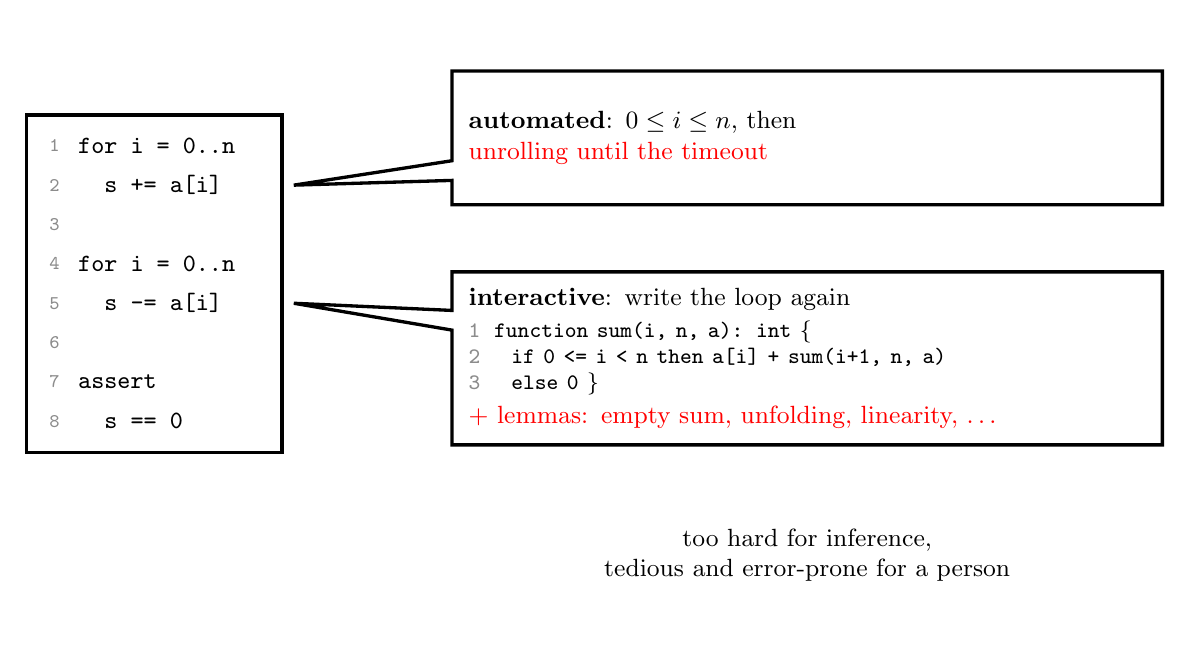
\begin{tikzpicture}
    \useasboundingbox (0,0) rectangle (14.4,7.6);
    \program{0.1}{6.6}{8}{for i = 0..n, \ \ s += a[i], {}, for i = 0..n, \ \ s -= a[i], {}, assert, \ \ s == 0}
    \node[bubble, text width=8.6cm, align=left, callout absolute pointer={($(P |- L2.east)+(0.15,0)$)}] at (9.9,6.2) {\textbf{automated}: $0 \le i \le n$, then\\ \bad{unrolling until the timeout}};
    \node[bubble, text width=8.6cm, align=left, font=\small, callout absolute pointer={($(P |- L5.east)+(0.15,0)$)}] at (9.9,3.4) {\textbf{interactive}: write the loop again\\[2pt]
        {\ttfamily\footnotesize\begin{tabular}{@{}r@{\hspace{5pt}}l@{}}
          \color{black!45}1 & function sum(i, n, a): int \{\\
          \color{black!45}2 & \ \ if 0 <= i < n then a[i] + sum(i+1, n, a)\\
          \color{black!45}3 & \ \ else 0 \}
        \end{tabular}}\\[2pt]
        \bad{+ lemmas: empty sum, unfolding, linearity, \ldots}};
    \node[align=center, font=\small, text width=8.6cm] at (9.9,0.9) {too hard for inference,\\ tedious and error-prone for a person};
  \end{tikzpicture}
\end{frame}

\cpa{26}
\cpa{7}

% why LLMs work: a good representation and knowing the solution, which motivates the claims
\cpa{12}

\claims{0}

% =====================================================================================================================
% claim 1: invariants are the wrong representation -> TEQs
\claims{1}

\begin{frame}
  \frametitle{\only<1>{Invariants}\only<2>{A much better explanation}}
  \begin{tikzpicture}
    \useasboundingbox (0,0) rectangle (14.4,7.4);
    \program{0.1}{6.4}{7}{while i < n, \ \ a[i] := z, \ \ i := i + 1, {}, assert, \ \ i == n \&\&, \ \ a[k] == z}
    \only<1>{
      \node[bubble, callout absolute pointer={($(P |- L1.east)+(0.15,0)$)}, text=cred] at (10.4,6.8) {$0 \le i \le n$};
      \node[bubble, callout absolute pointer={($(P |- L3.east)+(0.15,0)$)}, text=cred] at (10.4,4.7) {$\forall j.\ 0 \le j < i \Rightarrow a[j] = z$};
      \node[bubble, callout absolute pointer={($(P |- L6.east)+(0.15,0)$)}, text=cred] at (10.4,1.8) {lemma:\\ $i \le n \wedge \neg(i < n) \Rightarrow i = n$};}
    \only<2>{
      \node[bubble, callout absolute pointer={($(P |- L1.east)+(0.15,0)$)}, text=cblue] (b1) at (10.4,6.8) {$i$ counts from $0$ to $n$};
      \node[bubble, callout absolute pointer={($(P |- L3.east)+(0.15,0)$)}, text=cblue] (b2) at (10.4,4.7) {$a$ is set to $z$ \textcolor{cgreen}{\bfseries at all earlier $i$}};
      \draw[cgreen, very thick, -{Stealth[length=2.5mm]}] (b2.east) -- ++(0.35,0) |- (b1.east);
      \node[bubble, callout absolute pointer={($(P |- L6.east)+(0.15,0)$)}, text=cblue] at (10.4,1.8) {lemma:\\ a counter from $0$ to $n$ ends at $n$};}
  \end{tikzpicture}
\end{frame}

\begin{frame}{Trace equation systems}
  \begin{tikzpicture}
    \useasboundingbox (0,0) rectangle (14.4,7.4);
    \program{0.1}{6.4}{7}{while i < n, \ \ a[i] := z, \ \ i := i + 1, {}, assert, \ \ i == n \&\&, \ \ a[k] == z}
    \node[bubble, callout absolute pointer={($(P |- L1.east)+(0.15,0)$)}] (b1) at (10.4,6.8) {$I = \concept{\mathsf{counter}(0, 1, n)}$};
    \node[bubble, callout absolute pointer={($(P |- L2.east)+(0.15,0)$)}] (b2) at (10.4,4.7) {$A = \concept{\mathsf{stores}(a, {\color{cgreen}\bl{I}}, \bl{\mathsf{consts}(n, z)})}$};
    \draw[cgreen, very thick, -{Stealth[length=2.5mm]}] (b2.east) -- ++(0.35,0) |- (b1.east);
    \only<1>{\node[bubble, callout absolute pointer={($(P |- L6.east)+(0.15,0)$)}] at (10.4,1.8) {$\textcolor{cpurple}{\cur(}\concept{\mathsf{counter}(0, 1, n)}\textcolor{cpurple}{)} = n$};}
    \only<2>{\node[bubble, callout absolute pointer={($(P |- L7.east)+(0.15,0)$)}, align=left] at (10.4,1.8) {$\textcolor{cpurple}{\cur(}\concept{\mathsf{stores}(a, ks, vs)}\textcolor{cpurple}{)}[k] =$\\
        \quad $\mathsf{if}\ k \in ks\ \mathsf{then}\ vs[\mathsf{indexof}(k, ks)]$\\ \quad $\mathsf{else}\ a[k]$};}
  \end{tikzpicture}
\end{frame}

\begin{frame}{Variable-modular, not state-modular}
  \[
    x_n = \cur(X) \quad \text{where}
  \]
  \[
    X = \mathsf{trace}(x_0,\ \mathsf{for}\ \underbrace{\bl{K}, \bl{Y}}_{\text{dependencies}}\ \mathsf{do}\ x, k, y
      \mapsto \underbrace{u(x, k, y)}_{\text{update}})
  \]
  \vspace{0.3em}
  \begin{itemize}
    \item \concept{CHCs}: a loop is a relation on \emph{states}
    \item \concept{TEQs}: a loop is what each \emph{variable computes} over the iterations
    \item the loop is its own specification: \good{sound, relatively complete}
    \item program fragments get \good{names}: counter, stores, sums --- knowledge about them is reusable
  \end{itemize}
\end{frame}

% =====================================================================================================================
% claim 2: insight belongs in reusable lemmas -> the database; AI should make tools
\claims{2}

\cpa{35}

% the first example again: every step is a lemma of the database
\begin{frame}{Array initialization, by lemmas}
  \begin{tikzpicture}
    \useasboundingbox (0,0) rectangle (14.4,7.4);
    \program{0.1}{6.4}{7}{while i < n, \ \ a[i] := z, \ \ i := i + 1, {}, assert, \ \ i == n \&\&, \ \ a[k] == z}
    \node[bubble, callout absolute pointer={($(P |- L1.east)+(0.15,0)$)}] at (10.4,6.6)
      {$\mathsf{trace}(0, \mathsf{for}\ \bl{K}\ \mathsf{do}\ i, k \mapsto i + 1)$\\ $\rw \concept{\mathsf{counter}(0, 1, n)}$\\
       {\footnotesize\color{black!55} lemma \textsf{counter\_def}}};
    \node[bubble, callout absolute pointer={($(P |- L2.east)+(0.15,0)$)}] at (10.4,4.3)
      {$\mathsf{trace}(a, \mathsf{for}\ \bl{K}, \bl{I}\ \mathsf{do}\ a', k, i \mapsto a'[i := z])$\\ $\rw \concept{\mathsf{stores}(a, \bl{I}, \bl{\mathsf{consts}(n, z)})}$\\
       {\footnotesize\color{black!55} definition \textsf{stores}, lemma \textsf{maps\_const}}};
    \node[bubble, callout absolute pointer={($(P |- L7.east)+(0.15,0)$)}] at (10.4,1.7)
      {$a'[k] \rw \mathsf{if}\ 0 \le k < n\ \mathsf{then}\ z\ \ldots$\\ $\rw z$\\
       {\footnotesize\color{black!55} lemmas \textsf{current\_stores}, \textsf{occurs\_counter\_up},\\ \textsf{earlier\_consts}}};
    \node[align=center, font=\small] at (2.4,0.6) {\good{every step a database lemma},\\ none for the program};
  \end{tikzpicture}
\end{frame}

\begin{frame}{Routine, not trivial --- as TEQs}
  \begin{tikzpicture}
    \useasboundingbox (0,0) rectangle (14.4,7.4);
    \program{0.1}{6.4}{8}{for i = 0..n, \ \ s += a[i], {}, for i = 0..n, \ \ s -= a[i], {}, assert, \ \ s == 0}
    \node[bubble, callout absolute pointer={($(P |- L2.east)+(0.15,0)$)}] at (10.4,6.4) {$\mathsf{trace}(s_0, \mathsf{for}\ \bl{K}\ \mathsf{do}\ s, k \mapsto s + a[k])$\\
        $\rw \concept{\mathsf{sums}(s_0, \mathsf{selects}(a, \bl{K}))}$};
    \node[bubble, callout absolute pointer={($(P |- L5.east)+(0.15,0)$)}] at (10.4,4.0) {$\mathsf{trace}(s_1, \mathsf{for}\ \bl{K}\ \mathsf{do}\ s, k \mapsto s - a[k])$\\
        $\rw s_1 - \concept{\mathsf{sum}(\mathsf{selects}(a, \bl{K}))}$};
    \node[bubble, callout absolute pointer={($(P |- L8.east)+(0.15,0)$)}] at (10.4,1.5) {linearity: $s_0 + \mathsf{sum}(\ldots) - \mathsf{sum}(\ldots) = s_0$\\
        \good{no auxiliary function, no program lemma}};
  \end{tikzpicture}
\end{frame}

\cpa{41}

\begin{frame}{Two obvious ways to use AI}
  \begin{columns}[T]
    \begin{column}{0.48\textwidth}
      \textbf{AI as the verifier}
      \begin{itemize}
        \item ``model checking is dead''
        \item \bad{no trust}, no cross-check
        \item the answer is only as good as the last prompt
      \end{itemize}
    \end{column}
    \begin{column}{0.48\textwidth}
      \textbf{AI as the proof generator}
      \begin{itemize}
        \item Lean, Leanstral, \ldots: the proof is checked
        \item \bad{cost paid case by case}
        \item proofs at the level of \bad{assembler}
      \end{itemize}
    \end{column}
  \end{columns}
  \vspace{1.2em}
  \begin{center}
    both apply generative AI \emph{per program}
  \end{center}
\end{frame}

% the generated proof (CPA.pdf, slide 61), then the same theorem with a better tool
\cpa{61}

% the example of CPA.pdf slides 58 to 61, redone in Lean 4.34.1 (checked): one line with grind
\begin{frame}[fragile]{The same proof, with a better tool}
  \begin{columns}[T]
    \begin{column}{0.55\textwidth}
\begin{lstlisting}
inductive Tree (α : Type) where
  | leaf : Tree α
  | node : Tree α → α → Tree α → Tree α

def toList : Tree α → List α
  | leaf => []
  | node l x r => toList l ++ [x] ++ toList r

def BST [LT α] : Tree α → Prop
  | leaf => True
  | node l x r => (∀ y ∈ toList l, y < x) ∧
      (∀ y ∈ toList r, x < y) ∧ BST l ∧ BST r

def rotateLeft : Tree α → Tree α
  | node l x (node rl y rr) =>
      node (node l x rl) y rr
  | t => t
\end{lstlisting}
    \end{column}
    \begin{column}{0.43\textwidth}
\begin{lstlisting}[firstnumber=19]
theorem rotateLeft_BST [LT α]
    {l rl rr : Tree α} {x y : α}
    (lt_trans : ∀ {a b c : α},
       a < b → b < c → a < c)
    (h : BST (node l x
            (node rl y rr))) :
    BST (rotateLeft (node l x
            (node rl y rr))) := by
  grind [rotateLeft, BST, toList]
\end{lstlisting}
      \vspace{0.6em}
      \begin{itemize}\small
        \item \good{one line}, checked by Lean
        \item the generated proof did the case analysis \bad{by hand}
        \item the insight is in the \concept{tool} (\texttt{grind}), not in the proof
      \end{itemize}
    \end{column}
  \end{columns}
\end{frame}

\begin{frame}{Thesis: AI should make tools}
  \begin{center}
  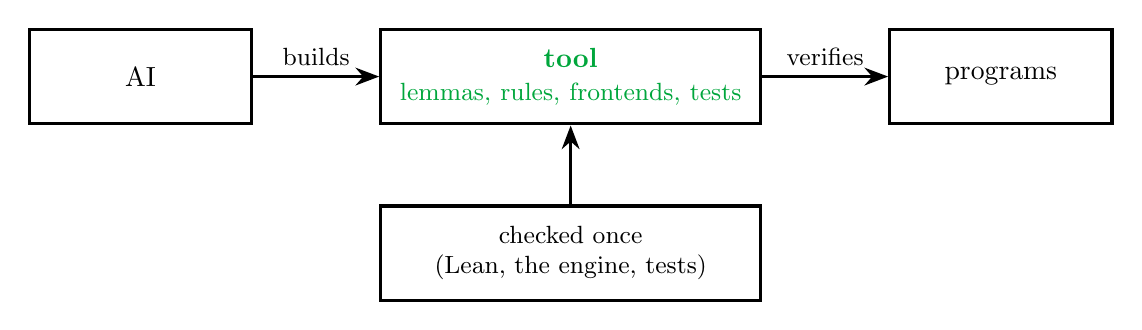
\begin{tikzpicture}
    \node[box, text width=2.4cm] (ai) {AI};
    \node[box, text width=4.4cm, right=1.6cm of ai, text=cgreen] (tool)
      {\bfseries tool\\ \mdseries\small lemmas, rules, frontends, tests};
    \node[box, text width=2.4cm, right=1.6cm of tool] (prog) {programs};
    \node[box, text width=4.4cm, below=1.0cm of tool, font=\small] (check) {checked once\\ (Lean, the engine, tests)};
    \draw[arrow] (ai) -- node[above, font=\small] {builds} (tool);
    \draw[arrow] (tool) -- node[above, font=\small] {verifies} (prog);
    \draw[arrow] (check) -- (tool);
  \end{tikzpicture}
  \end{center}
  \vspace{0.3em}
  \begin{itemize}
    \item the cost is paid \good{once per concept}, not once per program
    \item the trust is in a \good{checked artifact}, not in a language model
    \item AI writes what people find tedious: the lemma for every loop shape
  \end{itemize}
\end{frame}

\begin{frame}{The two threads meet}
  \begin{center}
  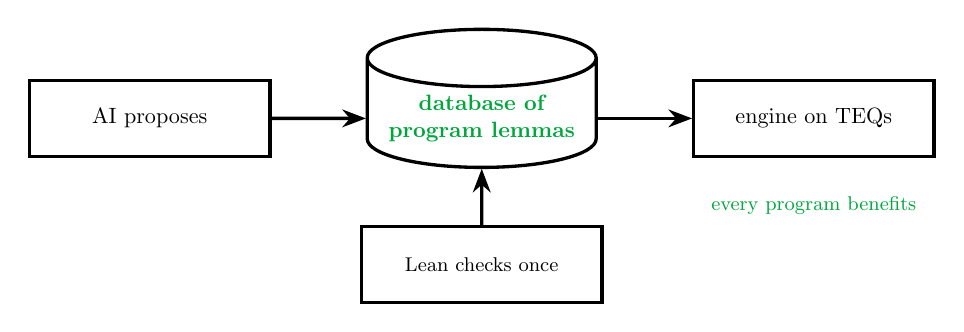
\begin{tikzpicture}[scale=0.8, transform shape]
    \node[box, text width=3.4cm] (ai) {AI proposes};
    \node[cylinder, shape border rotate=90, draw, very thick, aspect=0.25, align=center, text width=3.4cm,
          right=1.5cm of ai, text=cgreen, font=\bfseries] (db) {database of\\program lemmas};
    \node[box, text width=3.4cm, right=1.5cm of db] (engine) {engine on TEQs};
    \node[box, text width=3.4cm, below=0.9cm of db, font=\small] (lean) {Lean checks once};
    \draw[arrow] (ai) -- (db);
    \draw[arrow] (db) -- (engine);
    \draw[arrow] (lean) -- (db);
    \node[below=0.5cm of engine, font=\small, text=cgreen] {every program benefits};
  \end{tikzpicture}
  \end{center}
  \begin{itemize}
    \item TEQs make knowledge \concept{explicit and modular}: one lemma per loop shape
    \item what AI can write and a tool can check --- or LemmaCalc \cit{[iFM 25]}, without AI
  \end{itemize}
\end{frame}

\begin{frame}{How Cuvée is built}
  recent features, written by an AI agent (Claude Code) under direction:
  \begin{itemize}
    \item the lemma database: modules for counters, sums, stores, searches, sorting
    \item a new deduction engine (\texttt{-prove})
    \item state traces, the SV-LIB frontend, the ACSL annotations of SV-COMP
    \item examples, tests, and the documentation of every step
  \end{itemize}
  \vspace{0.6em}
  \textcolor{black!45}{% experience to be filled in by the speaker
  what worked, what did not}
\end{frame}

% =====================================================================================================================
% claim 3: reasoning must be incremental -> rewriting, state traces, partial descriptions
\claims{3}

\begin{frame}{Incremental reasoning on TEQs}
  \begin{itemize}
    \item rewriting with the database, \concept{one program fragment at a time}:\\
      partial results stay useful, nothing must be guessed up front
    \item the same representation carries far: nested loops, sorting, partitioning, merging
  \end{itemize}
  \vspace{0.5em}
  what makes it work beyond simple loops:
  \begin{enumerate}
    \item \concept{state traces}: variables that read each other
    \item \concept{partial descriptions}: proofs without a closed form
    \item \concept{a deduction engine}: congruence closure, simplex, lookup before decision
  \end{enumerate}
\end{frame}

\begin{frame}{State traces: variables that read each other}
  \begin{tikzpicture}
    \useasboundingbox (0,0) rectangle (14.4,7.4);
    \program{0.1}{6.4}{5}{while i < n, \ \ t := a[i], \ \ a[i] := b[i], \ \ b[i] := t, \ \ i := i + 1}
    \only<1>{
      \node[bubble, callout absolute pointer={($(P |- L3.east)+(0.15,0)$)}] at (10.4,6.0) {$A = \mathsf{trace}(a, \ldots \bl{B} \ldots)$\\ $B = \mathsf{trace}(b, \ldots \bl{A} \ldots)$\\
          \bad{one trace per variable: mutually recursive}};}
    \only<2->{
      \node[bubble, callout absolute pointer={($(P |- L3.east)+(0.15,0)$)}] at (10.4,6.0) {$S = \mathsf{trace}(a, b,\ \mathsf{for}\ \bl{I}\ \mathsf{do}\ a', b', i \mapsto$\\
          $a'[i := b'[i]],\ b'[i := a'[i]])$\\ \good{one trace per strongly connected component}};}
    \only<3>{
      \node[bubble, callout absolute pointer={($(P |- L4.east)+(0.15,0)$)}] at (10.4,2.8) {the lemmas see \concept{projections} of $S$:\\[2pt]
          $b'[k] \rw \mathsf{if}\ k \in \mathsf{prefix}(k, \bl{I})\ \ldots\ \mathsf{else}\ b[k]$\\[2pt]
          iteration $k$ reads what \good{no earlier iteration wrote}};}
  \end{tikzpicture}
\end{frame}

\begin{frame}{State traces: nested loops}
  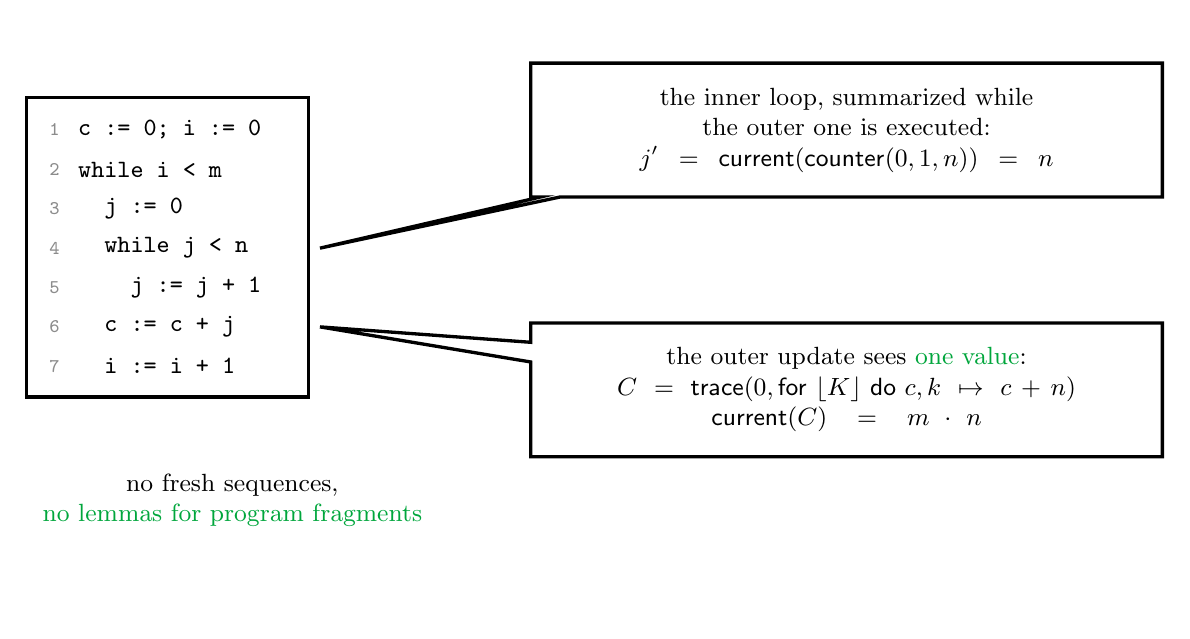
\begin{tikzpicture}
    \useasboundingbox (0,0) rectangle (14.4,7.4);
    \program{0.1}{6.6}{7}{c := 0; i := 0, while i < m, \ \ j := 0, \ \ while j < n, \ \ \ \ j := j + 1, \ \ c := c + j, \ \ i := i + 1}
    \node[bubble, callout absolute pointer={($(P |- L4.east)+(0.15,0)$)}] at (10.4,6.1) {the inner loop, summarized while\\ the outer one is executed:\\ $j' = \cur(\mathsf{counter}(0, 1, n)) = n$};
    \node[bubble, callout absolute pointer={($(P |- L6.east)+(0.15,0)$)}] at (10.4,2.8) {the outer update sees \good{one value}:\\ $C = \mathsf{trace}(0, \mathsf{for}\ \bl{K}\ \mathsf{do}\ c, k \mapsto c + n)$\\
        $\cur(C) = m \cdot n$};
    \node[align=center, font=\small] at (2.6,1.4) {no fresh sequences,\\ \good{no lemmas for program fragments}};
  \end{tikzpicture}
\end{frame}

\begin{frame}{Partial descriptions: binary search}
  \begin{tikzpicture}
    \useasboundingbox (0,0) rectangle (14.4,7.4);
    \program{0.1}{6.8}{10}{{lo, hi, i := 0, n, -1}, while lo < hi, \ \ mid := (lo + hi) / 2, \ \ if a[mid] < x, \ \ \ \ lo := mid + 1, \ \ else if x < a[mid], \ \ \ \ hi := mid, \ \ else, \ \ \ \ i := mid, \ \ \ \ break}
    \node[bubble, text width=6.9cm, callout absolute pointer={($(P |- L2.east)+(0.15,0)$)}] at (10.75,6.5) {exit: $hi \le lo \le p \le q \le hi$\\ \bad{open}: these lemmas are the program's own};
    \node[bubble, text width=6.9cm, callout absolute pointer={($(P |- L5.east)+(0.15,0)$)}] at (10.75,4.3) {no closed form for $lo$ and $hi$\\ \concept{abstraction}: grows up to a bound $b$\\
        $\rw \mathsf{incs}(x_0, b, \ldots)$};
    \node[bubble, text width=6.9cm, callout absolute pointer={($(P |- L7.east)+(0.15,0)$)}] at (10.75,1.9) {\concept{forward fact},\\ wherever the term occurs:\\ $x_0 \le b \Rightarrow \cur(\mathsf{incs}(x_0, b, \ldots)) \le b$};
  \end{tikzpicture}
\end{frame}

% =====================================================================================================================
% close
\begin{frame}{Questions for this community}
  \begin{columns}[T]
    \begin{column}{0.46\textwidth}
      \concept{CHCs}: state-modular\\
      {\small inductive invariants over integers}
    \end{column}
    \begin{column}{0.46\textwidth}
      \concept{TEQs}: variable-modular\\
      {\small loops that compute something}
    \end{column}
  \end{columns}
  \vspace{1em}
  \begin{itemize}
    \item TEQ summaries as \concept{loop acceleration} inside a CPA?
    \item TEQ normal forms as \concept{invariants in correctness witnesses}?
    \item \concept{shared frontends}: C, SV-LIB, Boogie, Dafny --- and Horn clauses as output
    \item which tasks does each side solve alone, and why?
  \end{itemize}
\end{frame}

\cpa{53}

\begin{frame}[plain]
  \centering\vfill
  {\fontsize{20}{26}\selectfont\bfseries Don't let AI verify programs.\\ Let it build the tools that do,\\[0.2em]
  \good{on a representation that makes their knowledge reusable.}}\\[2em]
  Thank you!\\[0.5em]
  {\small Trace Equation Systems for Program Verification \cit{[Coenen, Ernst, submitted 2026]}}
  \vfill
\end{frame}

\end{document}
